%Dokument til projektafgrænsningen
\section{Projektafgrænsning}

Vi har planlagt at arbejde med en kanon som skal kunne rotere 360 grader, samt have et vinkelinterval til affyring af kanonen på mindst 100 grader. Den fjernstyrede kanon skal være i stand til at modtage information fra et kontrolmodul. Dette skal ske ved brug af en bluetooth enhed eller et andet trådløst kommunikationsmodul. Der skal altså laves en mikrocontroller som kan styre kanonen gennem disse trådløse moduler ved at få kommandoer fra et kontrolmodul.\\

\begin{figure}[H]
\centering
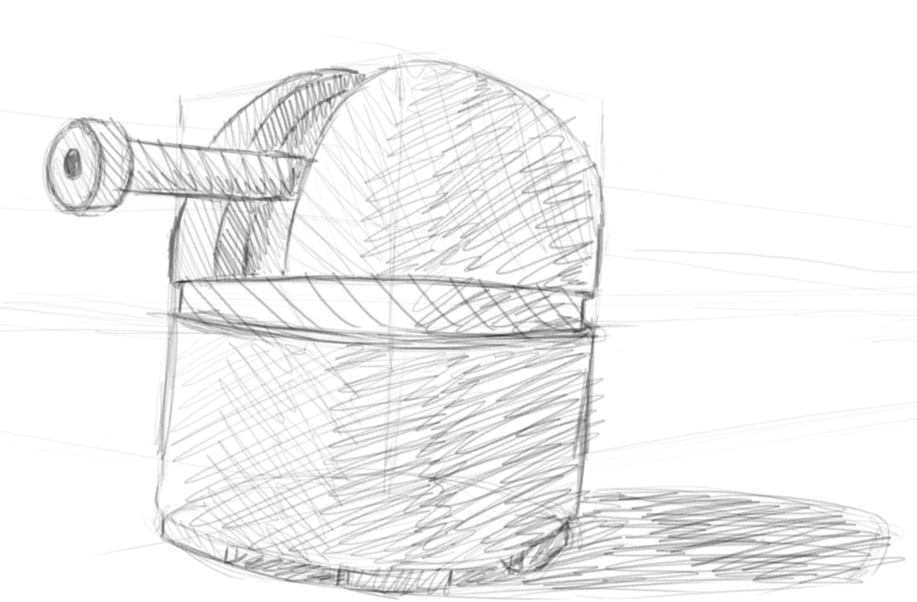
\includegraphics[scale=0.4]{Billeder/Koncept_turret.png}
\caption{Koncept af kanon.}
\label{fig:KonceptKanon}
\end{figure}

Selve kanons affyringsmekanisme laves enten med en “airsoft” pneumatisk gearkasse, hvor en DC motor bruges til at trække en fjeder op. Denne fjeder laver et lufttryk i gearkassens trykkammer som kan bruges til at skyde et projektil afsted. Selve robottens krop laves vha. 3D print af de enkelte komponenter, der sættes sammen med enten lim eller skruer. \\

Til udarbejdningen af det fysikvidenskabelige dokumentation kan der påmonteres forskellige afstandssensorer, som bruges til at måle projektilets hastighed. Derudover kan der alternativt måles, hvor langt projektilet bliver affyret for så, at kunne beregne dets hastighed, hvis affyringsvinklen er kendt.

\begin{figure}[H]
\centering
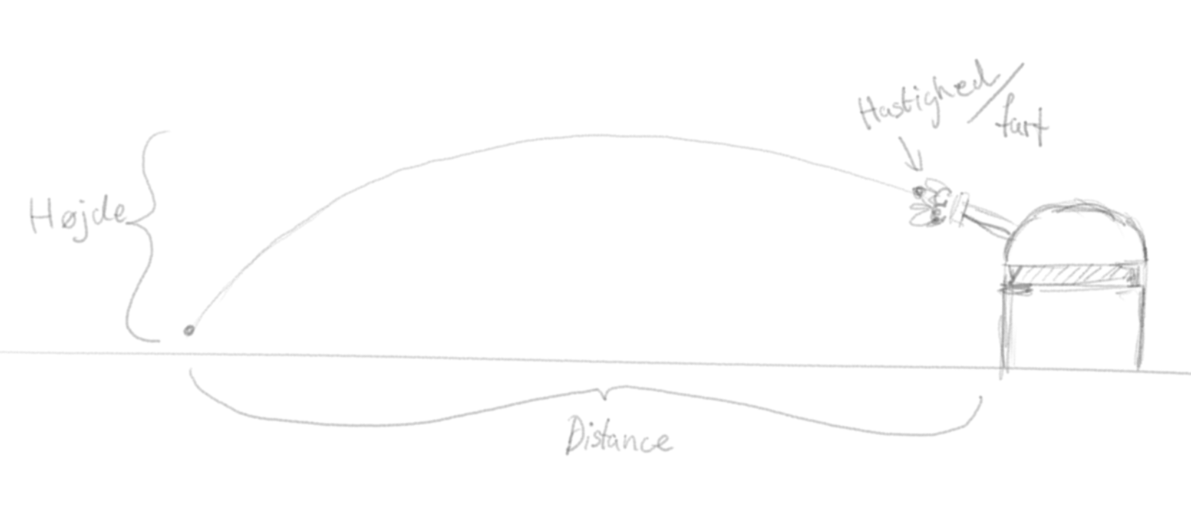
\includegraphics[scale=0.4]{Billeder/Fysik_koncept.png}
\caption{Fysik relevant til kanonen.}
\label{fig:FysikKoncept}
\end{figure}